\documentclass[10pt]{beamer}

%PTBR
%\usepackage[brazilian]{babel}
\usepackage[utf8]{inputenc}
\usepackage[T1]{fontenc}
\usepackage{bm}
\usepackage{graphicx}
\usepackage[absolute,overlay]{textpos} %pacote para posicionar o logo na primeira página
%\usepackage[dvipsnames]{xcolor}

%\usepackage{enumitem}

\usetheme[progressbar=frametitle]{metropolis}
\usepackage{appendixnumberbeamer}

\usepackage{booktabs}
\usepackage[scale=2]{ccicons}

\usepackage{pgfplots}
\usepgfplotslibrary{dateplot}

\usepackage{xspace}
\newcommand{\themename}{\textbf{\textsc{metropolis}}\xspace}

\newcommand{\induceint}{\ensuremath{\Imc_{\Amc^{*}, \Tmc}}}
\newcommand{\fullminmod}{\ensuremath{\Imc_{\Amc^{*}, \Tmc}} \cup \Imc_{\min}(\Tmc)}

\usepackage{bussproofs}

\usepackage{Macros}

%\definecolor{teal}{rgb}{0.0, 0.5, 0.5}
%\definecolor{darkorange}{rgb}{1.0, 0.55, 0.0}

\title{On Model Recovery}

\titlegraphic{%
  \begin{picture}(0,0)
    \put(305,-120){\makebox(0,0)[rt]{
\includegraphics[width=6cm]{img/logos.png}}}
  \end{picture}}

\date{\today}
\author{Igor de Camargo e Souza Câmara}
\institute{University of São Paulo}

\begin{document}

\begin{frame}[plain]
  \titlepage
\end{frame}

\begin{frame}[fragile]{Motivation}
  \begin{itemize}
    \item Edge upgrades may break the model, 
    \item Goal: recover the model property with as little disturbance as possible,
    \item Preserve an invariant -- \textbf{pre canonicity}.
  \end{itemize}
\end{frame}

\begin{frame}[fragile]{Pre canonicity}

  {\Large Pre Canonicity}
  
  \begin{enumerate}
    \item Required neighbors must be maximal to the root's type.
    \item Fixing the edges, there are no smaller models (\wrt concept membership) sharing the same domain.
  \end{enumerate}
\end{frame}

\begin{frame}[fragile]{Pre canonicity}
{\Large (1) Required neighbors must be maximal to the root's type.}
\begin{center}
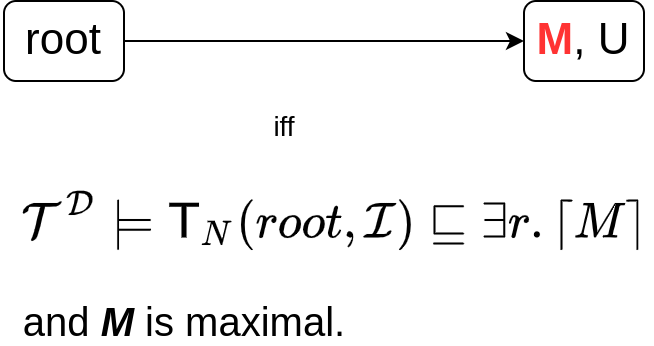
\includegraphics[scale=.35]{img/invariant_1.png}
\end{center}
\end{frame}

\begin{frame}[fragile]{Pre canonicity}
  \large (2) Fixing the edges, there are no smaller models (\wrt concept membership) sharing the same domain.
  \begin{center}
  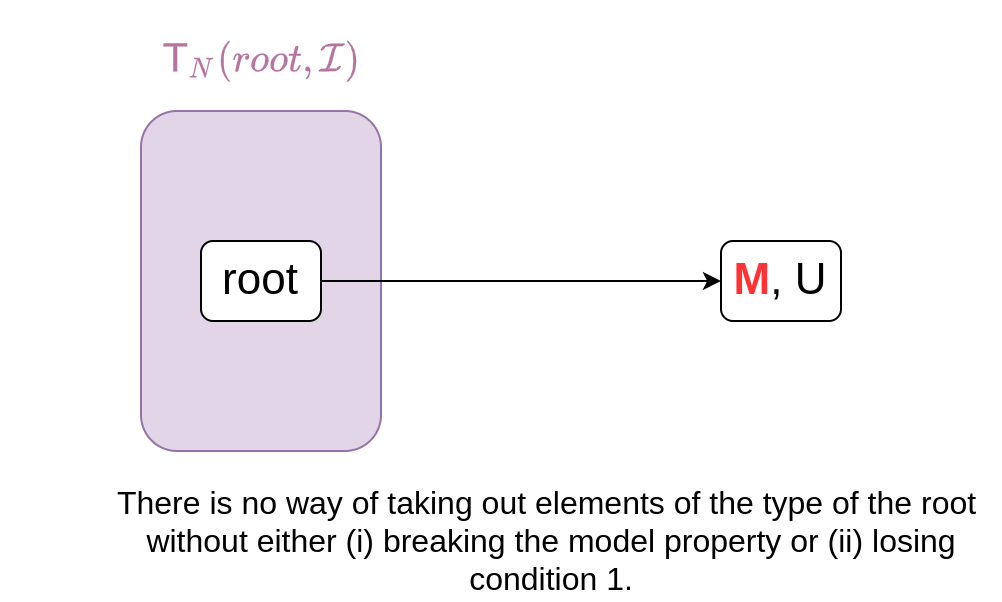
\includegraphics[scale=.3]{img/invariant_2.png}
  \end{center}
\end{frame}

\begin{frame}[fragile]{Extra condition -- Building from the upgraded interpretation}

  \begin{itemize}
  \item We must also ensure that the recovered model is not arbitrary, \ie, that it is a recovery over the original upgraded interpretation.
  \item This means that membership and edges should be preserved when possible \dots 
  \item \dots and all edges that move should move to concepts of the same typicality (\eg, moving $(M, {\color{red}\Umc})$ to $(N, {\color{red}\Umc})$).
\end{itemize}

\end{frame}

\begin{frame}[fragile]{Example 1}
  \begin{center}
  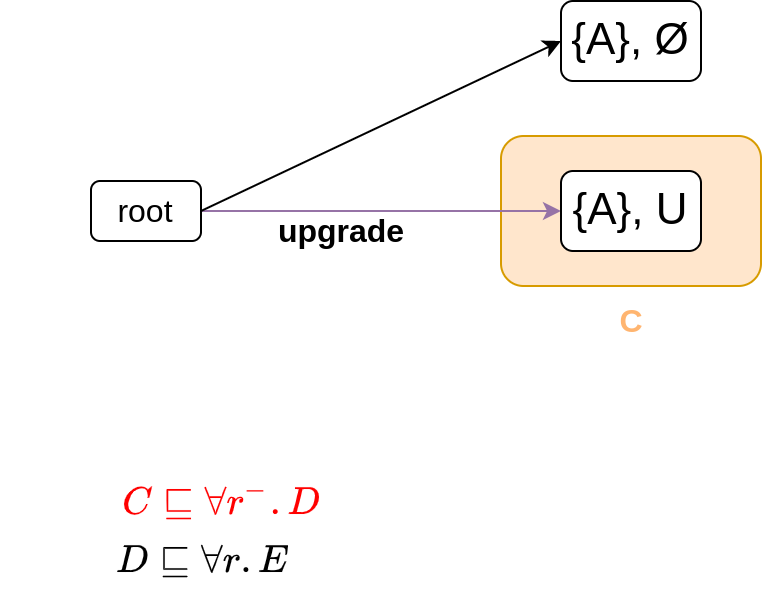
\includegraphics[scale=.3]{img/ex1_1.png}
  \end{center}
\end{frame}

\begin{frame}[fragile]{Example 1}
  \begin{center}
  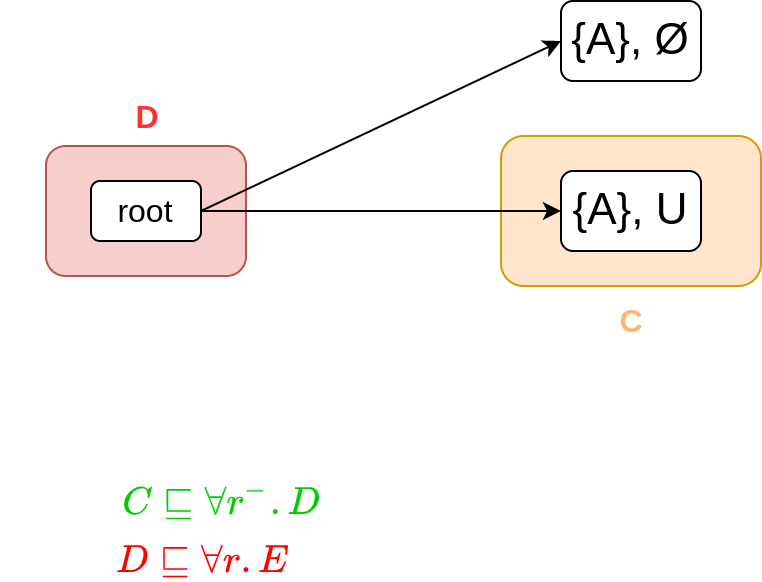
\includegraphics[scale=.3]{img/ex1_2.png}
  \end{center}
\end{frame}

\begin{frame}[fragile]{Example 1}
  \begin{center}
  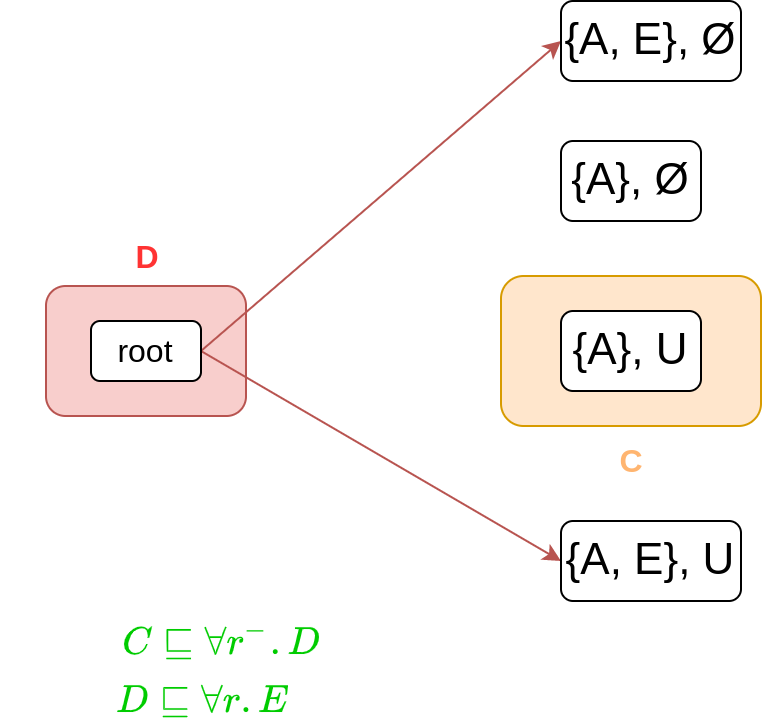
\includegraphics[scale=.3]{img/ex1_3.png}
  \end{center}
\end{frame}

\begin{frame}[fragile]{Example 2 -- Multiple Recoveries}
  \begin{itemize}
    \item The $root$ belonging to $D$ is a kind of \emph{artifact} from the upgrade procedure.
    \item It was required because the $root$ was connected to $(\{A\}, \Umc) \in C$, but this edge was later erased.
    \item This cannot be avoided -- taking $D$ out out hurt maximality \wrt neighbors. Further downgrading the edge would take us back to the initial situation.
  \end{itemize}
\end{frame}

\begin{frame}[fragile]{Example 2}
  \begin{center}
  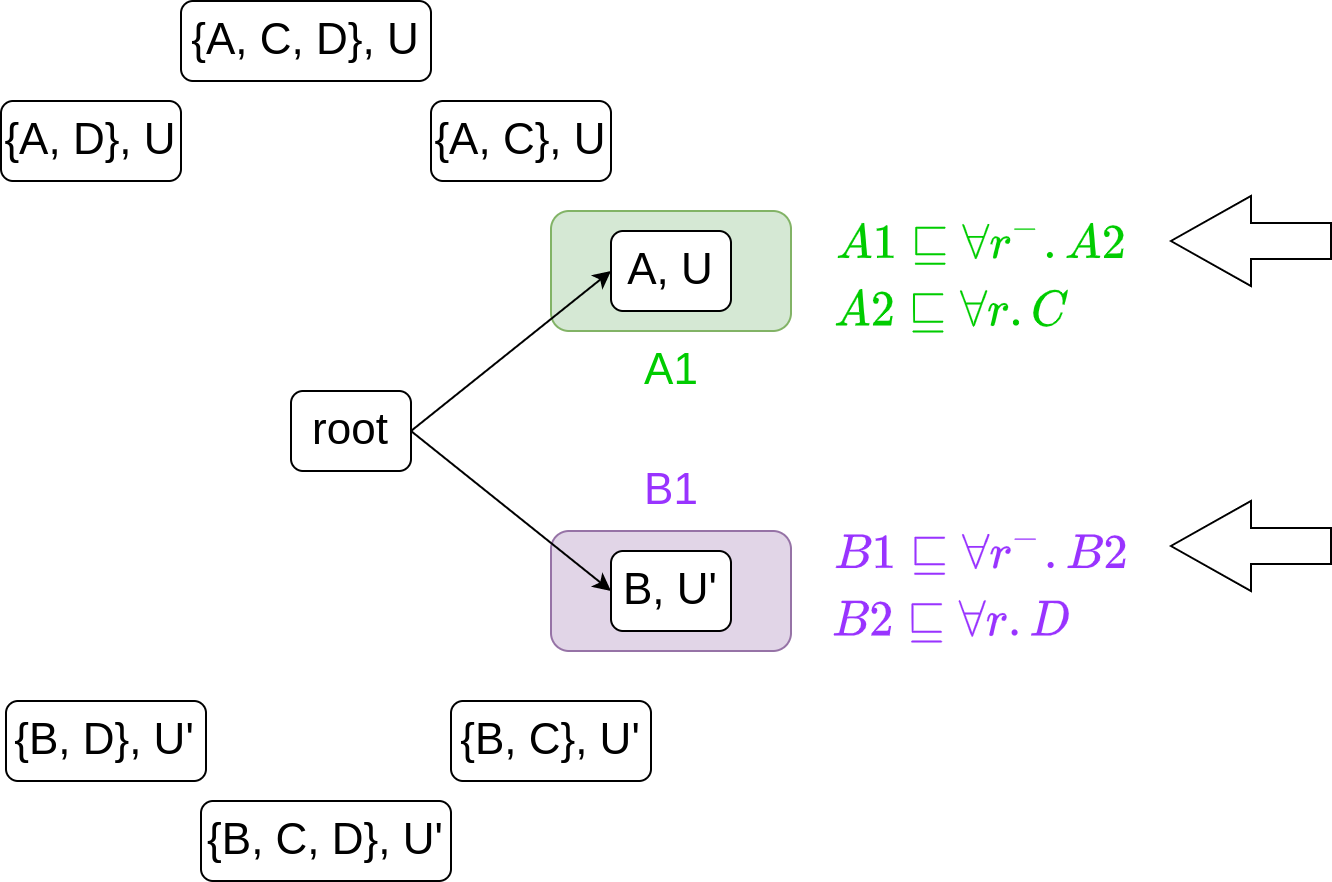
\includegraphics[scale=.25]{img/ex_1.png}
  \end{center}
\end{frame}

\begin{frame}[fragile]{Example 2 }
  \begin{center}
  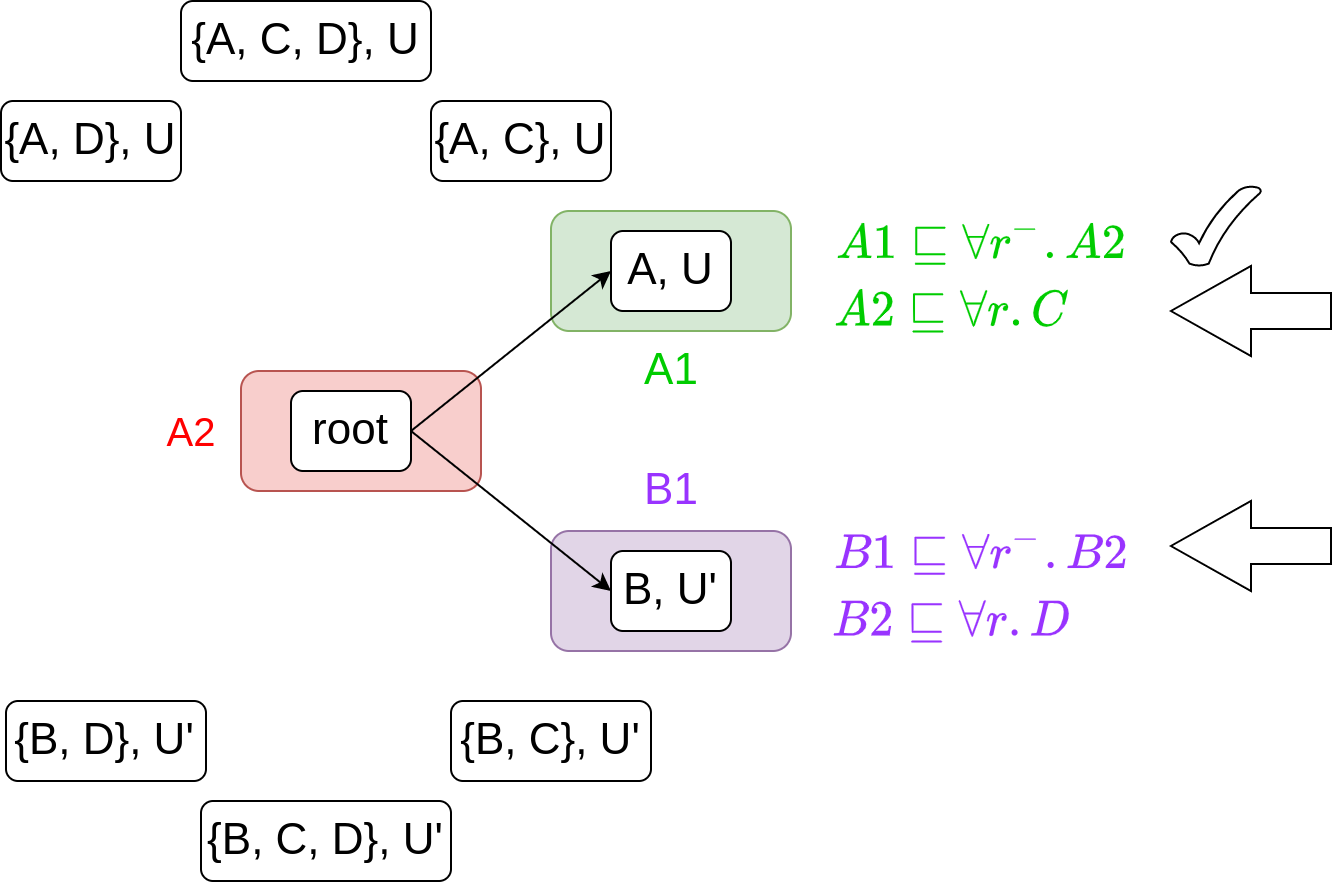
\includegraphics[scale=.25]{img/ex2_2.png}
  \end{center}
\end{frame}

\begin{frame}[fragile]{Example 2 -- Solution 1}
  \begin{center}
  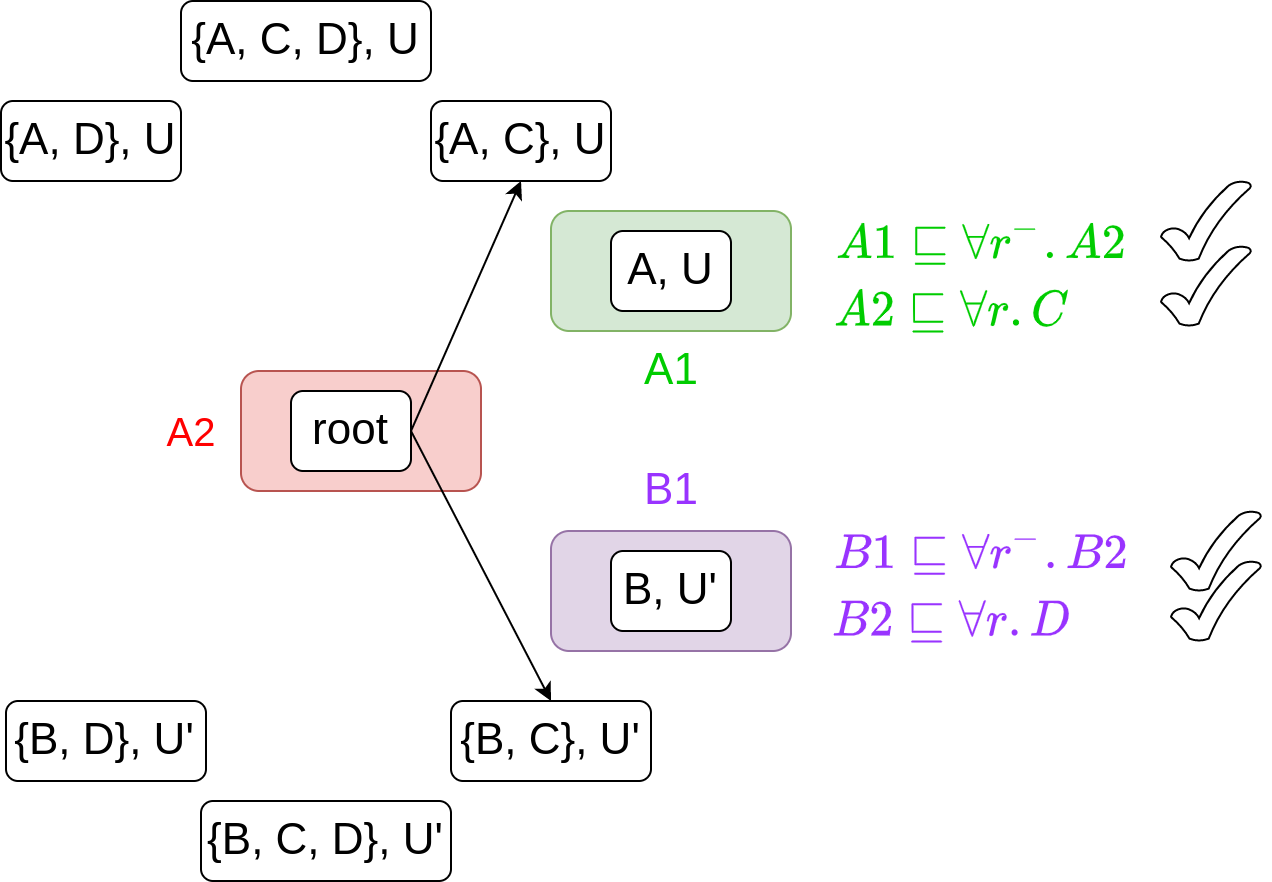
\includegraphics[scale=.25]{img/ex2_3.png}
  \end{center}
\end{frame}

\begin{frame}[fragile]{Example 2 -- Solution 2}
  \begin{center}
  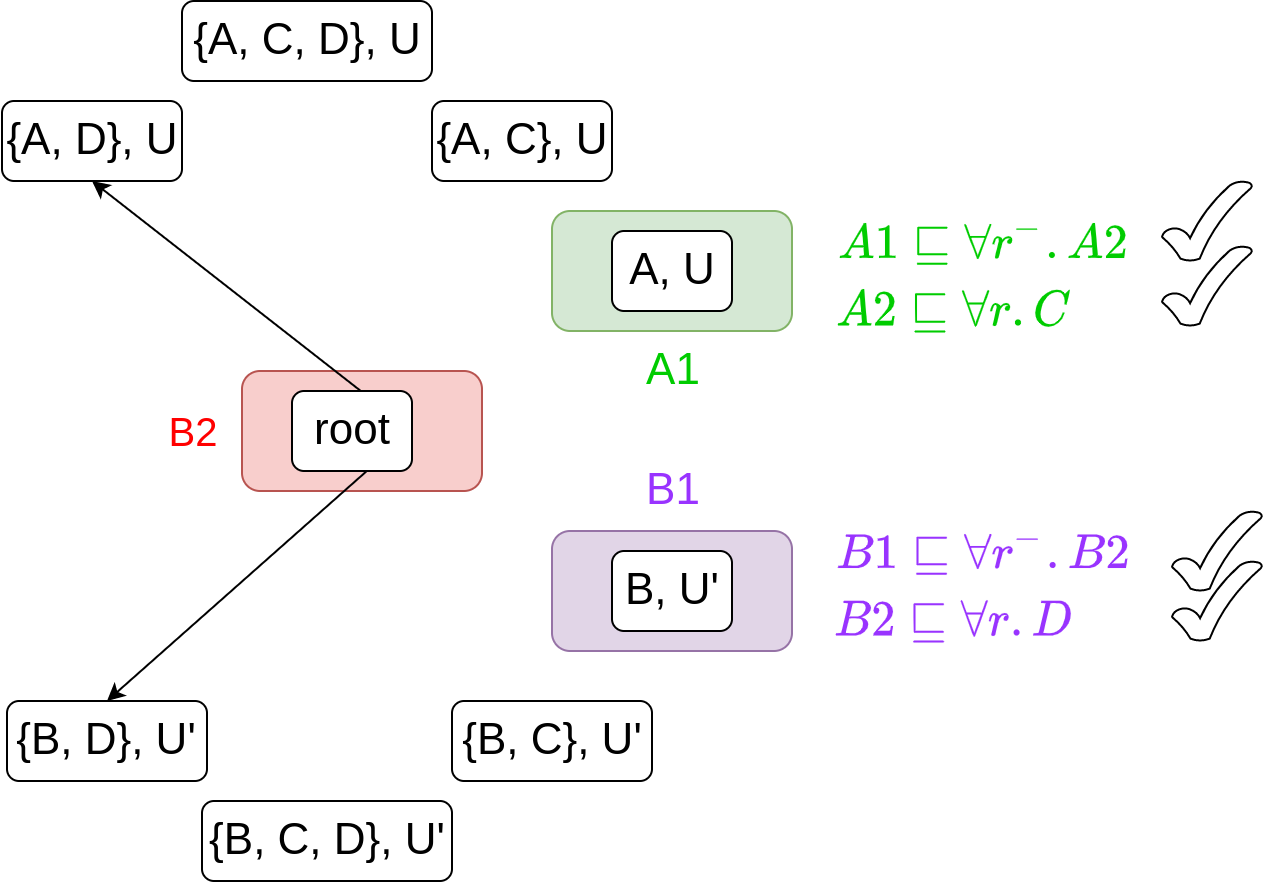
\includegraphics[scale=.25]{img/ex2_4.png}
  \end{center}
\end{frame}

\begin{frame}[fragile]{Example 2 -- Solution 3}
  \begin{center}
  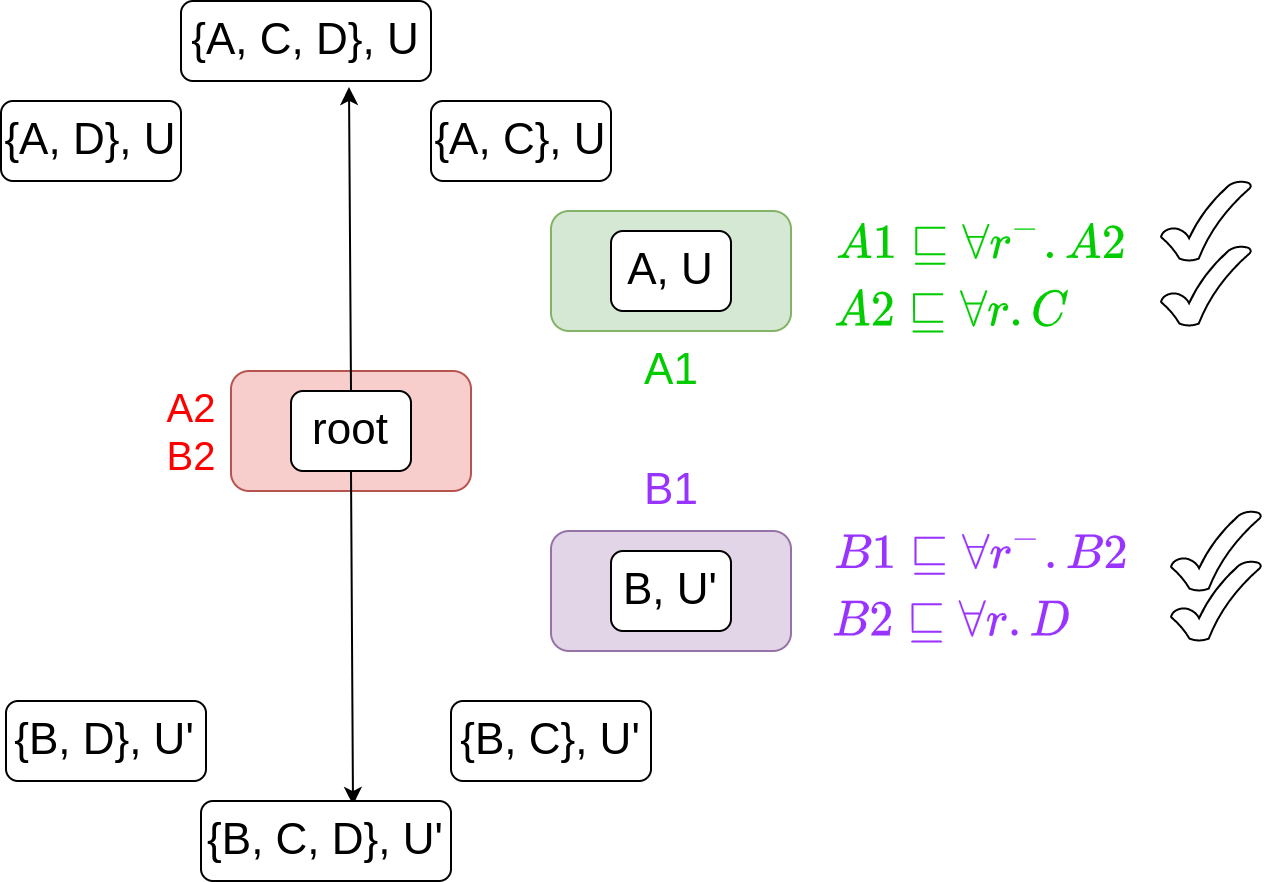
\includegraphics[scale=.25]{img/ex2_5.png}
  \end{center}
\end{frame}

\begin{frame}[fragile]{Comments on Example 2}

  \begin{itemize}
    \item Procedurally, recovering the model property is applying several \textbf{conflict resolution rules} to address \textbf{violations}.
    \item Solving one violation can dissolve others indirectly (by taking away edges that caused them).
    \item Essentially, the order in which one apply the conflict resolution rules may affect the outcome, and there is no way to circumvent this.
  \end{itemize}

\end{frame}

\begin{frame}[fragile]{Two ways of capturing this idea}
  \begin{itemize}
    \item A \textbf{semantic approach} captures how the models look like.
    \item A \textbf{procedural approach} captures a (non-deterministic) procedure to get from $\Imc$ to some $\Jmc$.
  \end{itemize}
\end{frame}

\begin{frame}[fragile]{Two ways of capturing this idea}
  \begin{itemize}
    \item A \textbf{semantic approach} captures how the models look like.
    \item A \textbf{procedural approach} captures a (non-deterministic) procedure to get from $\Imc$ to some $\Jmc$.
  \end{itemize}
\end{frame}

\begin{frame}[fragile]{The semantic approach}

  For an upgraded interpretation $\Imc$, a recovered model $\Jmc$ has to conform to the following properties... 

  \begin{enumerate}
    \item It must be a model of $\Kmc$ (satisfaction \wrt typicality models), \pause
    \item It should be an enlargement (\wrt concept membership) of $\Imc$, \pause
    \item It should have the \emph{pre canonical} property, \ie, every maximal edge required by the KB should be represented in the model, and every edge of the model must be maximal \wrt the KB. \pause
    \begin{itemize}
      \item This should conform to the edges in $\Imc$ -- new edges landing $(N, \Umc)$ should be improvements of $(N', \Umc)$ -- the second dimension is kept intact.  \pause
      \item We only deal with the level of typicality of neighbors during the upgrade step, not during the recovery. \pause
    \end{itemize}
    \item It should be the (one of the) smallest model(s) to satisfy the properties. \pause
    \begin{itemize}
      \item This should prevent spurious, non-necessary membership. 
    \end{itemize}
\end{enumerate}

\end{frame}

\begin{frame}[fragile]{The semantic approach}

  (1) It must be a model of $\Kmc$ (satisfaction \wrt typicality models), \pause
   

  Formally we say... 

  \begin{equation*}
    \Jmc \models \Kmc
  \end{equation*}

\end{frame}

\begin{frame}[fragile]{The semantic approach}
  (2) It should be an enlargement (\wrt concept membership) of $\Imc$, \pause
   

  Formally we say... 

  \begin{equation*}
    \Ntype{e}{\Imc} \subseteq \Ntype{e}{\Jmc} \text{for every } e \in \Delta^{\Imc}
  \end{equation*}

  Additionally, we may postulate that the change needs to be kept within the \textbf{dependency set} of the root (\ie, whatever element outside of this set must remain the same).
\end{frame}

\begin{frame}[fragile]{The semantic approach (the long one)}
  (3) It should have the \emph{pre canonical} property, \ie, {\color{red}every maximal edge required by the KB should be represented in the model}, and every edge of the model must be maximal \wrt the KB. \pause
   
  Formally we say... 

  \begin{align*}
    \text{If } \Tmc^{\Dmc} \models & \setconj{\Ntype{\typel{M}{\Umc}}{\Jmc}} \sqcap \ELmaterialization{\Umc}  \sqsubseteq \exists r.\setconj{N} \text{ for a maximal } N \text{, then } \\ 
    & \text{(a) } (\typel{M}{\Umc}, \typel{N}{\Umc'} ) \in r^{\Jmc} \text{ } \forall \typel{N}{\Umc'} \textit{s.t. } \exists N'\subseteq N. (\typel{M}{\Umc}, \typel{N'}{\Umc'}) \in r^{\Imc} \text{, and}\\ 
    & \text{(b) }(\typel{M}{\Umc}, \typel{N}{\emptyset}) \in r^{\Jmc}
  \end{align*}
\end{frame}

\begin{frame}[fragile]{The semantic approach (the long one)}
  (3) It should have the \emph{pre canonical} property, \ie, every maximal edge required by the KB should be represented in the model, and {\color{red} every edge of the model must be maximal \wrt the KB}. \pause
   
  Formally we say... 

  \begin{align*}
    \text{If }&(\typel{M}{\Umc}, \typel{N}{\Umc'}) \in r^{\Imc}  \text{, then} \\
    & \Tmc^{\Dmc} \models \Ntype{\typel{M}{\Umc}}{\Jmc} \sqcap \ELmaterialization{\Umc} \sqsubseteq \exists r.\setconj{N} \text{ for a maximal } M \text{, and} \\
    & \exists N' \sqsubseteq N \textit{ s.t. } (\typel{M}{\Umc}, \typel{N'}{\Umc'}) \in r^{\Imc} \text{ or } \\
    & \Umc' = \emptyset 
  \end{align*}
\end{frame}

\begin{frame}[fragile]{The semantic approach}
  (4) It should be the (one of the) smallest model(s) to satisfy the properties. \pause
   
  Formally we say... 

  \begin{align*}
    \nexists \Jmc' = (\Delta^{\Imc}, \cdot^{\Imc}) \textit{ s.t. } \\
    r^{\Jmc'} = r^{\Jmc} \text{ and } \\ 
    \forall e \in \Delta^{\Imc}.\Ntype{e}{\Jmc'} \subseteq \Ntype{e}{\Jmc}
  \end{align*}
\end{frame}

\begin{frame}[fragile]{The procedural approach -- Intuition}
A set of rules to deal with \emph{violations}.
Those violations are not only axiom violations, but also deal with interpretations that do not conform to the properties outlined in the semantic approach.

$\Jmc$ is an \emph{improvement over} $\Imc$ iff it is generated by applying one of the rules to $\Imc$.

A series $\Imc_1, \dots, \Imc_k$ fixes $\Imc_1$ iff $\Imc^{i}$ is an improvement over $\Imc^{i+1}$ and $\Imc^{k}$ contains no violation.
\end{frame}

\end{document}


